\documentclass[10pt,conference]{IEEEtran}

\ifCLASSINFOpdf
	\usepackage[pdftex]{graphicx}
	%\graphicspath{{./figs/}}
	\DeclareGraphicsExtensions{.pdf,.jpeg,.png}
\else
	\usepackage[dvips]{graphicx}
	%\graphicspath{{./figs/}}
	\DeclareGraphicsExtensions{.eps}
\fi

\usepackage{listings}
\lstset{breaklines=true}
\lstset{extendedchars=false}
\usepackage[cmex10]{amsmath}
\usepackage[tight,footnotesize]{subfigure}
\usepackage{xcolor}
\usepackage[lined,ruled]{algorithm2e}

\usepackage[latin1]{inputenc}
\usepackage{tikz}
\usetikzlibrary{shapes}
\usetikzlibrary{arrows}

\usepackage[]{algorithm2e}

\newtheorem{property}{Property}
\newtheorem{proposition}{Proposition}
\newtheorem{theorem}{Theorem}
\newtheorem{conjecture}{Conjecture}
\newtheorem{question}{Question}
\newtheorem{definition}{Definition}
\newtheorem{corollary}{Corollary}

\makeatletter
\pgfdeclareshape{datastore}{
\inheritsavedanchors[from=rectangle]
\inheritanchorborder[from=rectangle]
\inheritanchor[from=rectangle]{center}
\inheritanchor[from=rectangle]{base}
\inheritanchor[from=rectangle]{north}
\inheritanchor[from=rectangle]{north east}
\inheritanchor[from=rectangle]{east}
\inheritanchor[from=rectangle]{south east}
\inheritanchor[from=rectangle]{south}
\inheritanchor[from=rectangle]{south west}
\inheritanchor[from=rectangle]{west}
\inheritanchor[from=rectangle]{north west}
\backgroundpath{
    %  store lower right in xa/ya and upper right in xb/yb
\southwest \pgf@xa=\pgf@x \pgf@ya=\pgf@y
\northeast \pgf@xb=\pgf@x \pgf@yb=\pgf@y
\pgfpathmoveto{\pgfpoint{\pgf@xa}{\pgf@ya}}
\pgfpathlineto{\pgfpoint{\pgf@xb}{\pgf@ya}}
\pgfpathmoveto{\pgfpoint{\pgf@xa}{\pgf@yb}}
\pgfpathlineto{\pgfpoint{\pgf@xb}{\pgf@yb}}
 }
}
\makeatother

\newcommand{\riham}[1]{{\color{red}{#1}}}
\newcommand{\james}[1]{{\color{blue}{#1}}}


\begin{document}

\title{Implementation and Visualization of A* Algorithm Based on Web Game "Eight-figure puzzles"}
\author{
\IEEEauthorblockN{Chengyuan Deng}
\IEEEauthorblockA{CS Department, Rutgers University\\ Piscataway, NJ, USA\\
Email: charren.d@rutgers.edu}
\and
\IEEEauthorblockN{Sagar Jain}
\IEEEauthorblockA{CS Department, Rutgers University\\Piscataway, NJ, USA\\
Email: sj735@rutgers.edu}
\and
\IEEEauthorblockN{Gauthamram Prabaharan}
\IEEEauthorblockA{CS Department, Rutgers University\\Piscataway, NJ, USA\\
Email: gauthamram.prabaharan@rutgers.edu}
}

\maketitle
\begin{abstract}
\textnormal{
A* algorithm, known as a heuristic algorithm with lower time and memory complexity comparing with other shortest path searching algorithms(e.g. Dijkstra's algorithm), enjoys widespread use in real time strategy games due to its performance and accuracy. In this project, A* algorithm will be implemented in the game "eight-figure puzzles", which is a strategy game in 2D grid, and the process of implementation will be visualized on a web page. Unsuspiciously, this project will be fun since the form of implementing an advanced algorithm by games is attracting and novel. The visualization of the process is helpful for students to grasp a better understanding on A* algorithm while having fun playing the games!
}
\end{abstract}
%\onecolumn \maketitle \normalsize \vfill

\IEEEpeerreviewmaketitle
%%%%%%%%%%%%%%%%%%%%%%%%%%%%%%%%%%%%%%%%%%%%%%%%%%%%%%%%%%%%%%%%%%%%%%%%%%%%%%%%%%%%%%%%%%%%%%%%%%%%%%%%%
\section{Project Description}\label{sec:1. Project Description}
%%%%%%%%%%%%%%%%%%%%%%%%%%%%%%%%%%%%%%%%%%%%%%%%%%%%%%%%%%%%%%%%%%%%%%%%%%%%%%%%%%%%%%%%%%%%%%%%%%%%%%%%%
\textnormal{
As mentioned in the abstract, the core component of this project is A* algorithm, based on which a real time strategy game called "eight-figure puzzles" will be developed and deployed online with HTML,CSS and JavaScript. The users can try to solve the game themselves, but meanwhile a visualization of solving the "eight-figure puzzles" game using A* algorithm will be provided on the web page to show the implementing process of A*. The type of this project is similar to type a and type b among those in posted sakai announcement, but we work more than what those types require since we actually develop a web application, which is more useful than just a sample or an animation. We are confident to complete this project by the deadline given the strong background of our group mates. The idea of the whole project is definitely novel as it integrates learning algorithm and playing games. The main stumbling block we can see temporarily is the web application for games. It's more complicated than just developing a web site or just developing a game. The timeline for this project will fit in stage2,stage3,stage4 respectively, we will complete the basic implementation of A* algorithm by stage2, the visualization and web application by stage3, and testing of the web application with optimization by stage4. We will reach the major milestone of this project by concentrating on the algorithm and studying advanced JavaScript for the web application.
}

The project has four stages: Gathering, Design, Infrastructure Implementation, and User Interface.

%\subsection{Stage1 - The Requirement Gathering Stage. } \label{sec:1	Requirement Gathering Stage. }
%\textnormal{
This project is designed with a realistic idea that includes potential real world scenarios,
with a description of the different user types along with their interactions with the system
as well as the system feedback to them, according to their information needs.
This stage also requires the specification of the different constraints and restrictions
that need to be enforced depending on the different types of user.
The deliverables for stage1 are as follows:
}


\begin{itemize}
\item{The general system description: }
The system of our project is composed of three parts: web application, A* algorithm and "eight-figure puzzles" game. Basically, relationship of the three parts is: The game is deployed on the web application and users can try to solve it; A* algorithm is introduced to solve the game; The web application will show the process of implementing A* algorithm to solve the game.
\item{The three types of users (grouped by their data access/update rights): }
Three types of user are considered in this project, the details are as follows:

    \begin{itemize}
    \item{Type1 ordinary game player: }
	For ordinary game player, they will certainly have access to the game and enjoy it. They may also have rights to see the result. But they are not allowed to view the process that the game is solved, nor are they qualified to change to visualization mode. 
    \item{Type2 advanced game player: }
	Once a user turns to an advanced game player, he certainly maintains all the right as ordinary game player, what's more, he can control the visualization mode and speed.
	\item{Type3 administrator: }
	Indubitably the administrator has the highest authority on the system. He can control and change everything.
    \end{itemize}
    
\item{The user's interaction modes: }
    \begin{itemize}
    \item{Game playing web page:}
    Left and right distributed, the left part will show the 2D grid of "eight-figure" puzzles, the right part contains a brief introduction of the initial status and the goal status.
    \item{visualization web page:}
    Left and right distributed, the left part is a canvas where the steps of A* algorithm will be shown, the right part includes a control bar of the visualization and a message bar showing the distance values of A* algorithm.
    \end{itemize}
\item{The real world scenario1: }
Game player update operations on the game

	\begin{itemize}
	\item{System Data Input for Scenario1: }
	An array of the eight numbers in each block by the designed order.
	\item{Input Data Types for Scenario1: }
	3*3 2D graph with 9 blocks, 8 of them are labeled with the designated number, the rest is blank.
	\item{System Data Output for Scenario1: }
	An array of the eight numbers in each block by the designed order after one or several steps in A* algorithm.
	\item{Output Data Types for Scenario1: }
	3*3 2D graph with 9 blocks, 8 of them are labeled with the number after updated, the rest is blank.
	\end{itemize}

\item{The real world scenario2: }
Please insert the real world scenarios in here, as follows.

	\begin{itemize}
	\item{System Data Input for Scenario2: }
	Click the button "step","run" and "pause". Change the frequency of updating steps by keyboard input.
	\item{Input Data Types for Scenario2: }
	Keyboard control, mouse control
	\item{System Data Output for Scenario2: }
	 Button "step" will show every searching step of A* algorithm and be paused automatically. Button "run" allows the algorithm continuing running and showing the results after clicking.  Input the intervals of updating steps to control the speed of visualization.
	\item{Output Data Types for Scenario2: }
	A spanning tree indicating the searching process of A* algorithm.
	\end{itemize}

\item{Project Time line}
   \begin{itemize}
	\item{Stage1 (Oct.27): }
	Requirement gathering, plan and division of work, knowledge of A* algorithm.
	\item{Stage2 (Nov.10): }
	System flow diagram containing a graphical representation and textual descriptions of the corresponding data transformations, high level pseudo code of A* algorithm, time and space complexity, knowledge of JavaScript on web application.
	\item{Stage3 (Nov.24): }
	Implementation of A* algorithm, web game application.
	\item{Stage4 (Dec.8): }
	Integrating, testing and optimization of the web application, writing the report, preparing presentation and codes.
	\end{itemize}
\item{Division of Labor: }
    \begin{itemize}
    
	\item{implementation of A*: }
	Sagar Jain, Gauthamram Prabaharan
	\item{web application: }
	Chengyuan Deng
	\item{deploy the game on website : }
	Chengyuan Deng
    \item{visualization: }
    Chengyuan Deng
    \item{testing: }
    Sagar Jain
    \item{evaluation: }
    Gauthamram Prabaharan
    \item{project report: }
    Chengyuan Deng
    \item{power point presentation: }
    Sagar Jain, Gauthamram Prabaharan
	\end{itemize}
\end{itemize}


\subsection{Stage1 - The Requirement Gathering Stage. }\label{sec:1 Requirement Gathering Stage. }
%%%%%%%
\textnormal{
This project is designed with a realistic idea that includes potential real world scenarios,
with a description of the different user types along with their interactions with the system
as well as the system feedback to them, according to their information needs.
This stage also requires the specification of the different constraints and restrictions
that need to be enforced depending on the different types of user.
The deliverables for stage1 are as follows:
}


\begin{itemize}
\item{The general system description: }
The system of our project is composed of three parts: web application, A* algorithm and "eight-figure puzzles" game. Basically, relationship of the three parts is: The game is deployed on the web application and users can try to solve it; A* algorithm is introduced to solve the game; The web application will show the process of implementing A* algorithm to solve the game.
\item{The three types of users (grouped by their data access/update rights): }
Three types of user are considered in this project, the details are as follows:

    \begin{itemize}
    \item{Type1 ordinary game player: }
	For ordinary game player, they will certainly have access to the game and enjoy it. They may also have rights to see the result. But they are not allowed to view the process that the game is solved, nor are they qualified to change to visualization mode. 
    \item{Type2 advanced game player: }
	Once a user turns to an advanced game player, he certainly maintains all the right as ordinary game player, what's more, he can control the visualization mode and speed.
	\item{Type3 administrator: }
	Indubitably the administrator has the highest authority on the system. He can control and change everything.
    \end{itemize}
    
\item{The user's interaction modes: }
    \begin{itemize}
    \item{Game playing web page:}
    Left and right distributed, the left part will show the 2D grid of "eight-figure" puzzles, the right part contains a brief introduction of the initial status and the goal status.
    \item{visualization web page:}
    Left and right distributed, the left part is a canvas where the steps of A* algorithm will be shown, the right part includes a control bar of the visualization and a message bar showing the distance values of A* algorithm.
    \end{itemize}
\item{The real world scenario1: }
Game player update operations on the game

	\begin{itemize}
	\item{System Data Input for Scenario1: }
	An array of the eight numbers in each block by the designed order.
	\item{Input Data Types for Scenario1: }
	3*3 2D graph with 9 blocks, 8 of them are labeled with the designated number, the rest is blank.
	\item{System Data Output for Scenario1: }
	An array of the eight numbers in each block by the designed order after one or several steps in A* algorithm.
	\item{Output Data Types for Scenario1: }
	3*3 2D graph with 9 blocks, 8 of them are labeled with the number after updated, the rest is blank.
	\end{itemize}

\item{The real world scenario2: }
Please insert the real world scenarios in here, as follows.

	\begin{itemize}
	\item{System Data Input for Scenario2: }
	Click the button "step","run" and "pause". Change the frequency of updating steps by keyboard input.
	\item{Input Data Types for Scenario2: }
	Keyboard control, mouse control
	\item{System Data Output for Scenario2: }
	 Button "step" will show every searching step of A* algorithm and be paused automatically. Button "run" allows the algorithm continuing running and showing the results after clicking.  Input the intervals of updating steps to control the speed of visualization.
	\item{Output Data Types for Scenario2: }
	A spanning tree indicating the searching process of A* algorithm.
	\end{itemize}

\item{Project Time line}
   \begin{itemize}
	\item{Stage1 (Oct.27): }
	Requirement gathering, plan and division of work, knowledge of A* algorithm.
	\item{Stage2 (Nov.10): }
	System flow diagram containing a graphical representation and textual descriptions of the corresponding data transformations, high level pseudo code of A* algorithm, time and space complexity, knowledge of JavaScript on web application.
	\item{Stage3 (Nov.24): }
	Implementation of A* algorithm, web game application.
	\item{Stage4 (Dec.8): }
	Integrating, testing and optimization of the web application, writing the report, preparing presentation and codes.
	\end{itemize}
\item{Division of Labor: }
    \begin{itemize}
    
	\item{implementation of A*: }
	Sagar Jain, Gauthamram Prabaharan
	\item{web application: }
	Chengyuan Deng
	\item{deploy the game on website : }
	Chengyuan Deng
    \item{visualization: }
    Chengyuan Deng
    \item{testing: }
    Sagar Jain
    \item{evaluation: }
    Gauthamram Prabaharan
    \item{project report: }
    Chengyuan Deng
    \item{power point presentation: }
    Sagar Jain, Gauthamram Prabaharan
	\end{itemize}
\end{itemize}




\subsection{Stage2 - The Design Stage. }\label{sec: 2:The Design Stage.}
%%%%%%%%%%%%%%%%%%%%%%%%%%%%%%%%%%%%%%%%%%%%%%%%%%%%%%%%%%%%%%%%%%%%%%%%%%%%%%%%%%%%%%%%%%%%%%%%%%%%%%%%%%
\textnormal{
The deliverables for this stage include the system flow diagram containing a graphical representation and textual descriptions of the corresponding data transformations, high level pseudo code of the overall system operation, and overall system time and space complexity.}

\begin{itemize}
\item{ }
Since the target of this project is an elaborate demonstration of A* algorithm in the form of "8-figure puzzle" game on a web site, the system should then be this web site. Distinct users, all regarded as game players, will enjoy playing the game along with viewing the process of implementing A* algorithm to solve the game, only that the advanced game players are qualified to control the visualization mode and speed.
\item{ }
Algorithms about web development and user interaction will not be discussed in this report. A* algorithm will be based on Javascript language and use data structures like array, hash table, priority queue,etc. The system design will also include an entity called "identity" recording the current user information and his authorization, will have attributes including "username", "password", "type", etc, and operations including "ChangePassword","Upgrade", etc, which help the system distinguish the user type and grant authorization accordingly.
\end{itemize}

Please insert your deliverables for Stage2 as follows:
\begin{itemize}
\item{  Short Textual Project Description. }
This project will be demonstrated in the form of a dynamic web site where canvas will be designed on the web page to make the visualization more attracting. The execution follow the flow of "home page-game page-visualization canvas-mode control", as shown more explicitly in figure 1.

The time complexity of A* depends on the heuristic. For the worst case of an unbounded search space, the number of nodes expanded is exponential in the depth of the solution d: $O(b^d)$, where b is the branching factor.

The space complexity of A* only is $O(n^2)$, the overall will vary with the web site status.

\item{ Flow Diagram. }
\begin{figure}[ht]
\centering
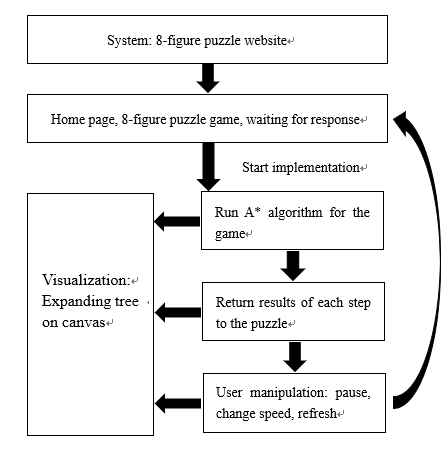
\includegraphics[width=3.13in]{figure1}
\label:{figure 1}
\end{figure}
Figure 1 indicates the execution diagram of the whole system, while the following figure 2 shows the flow diagram of A* algorithm.

\begin{figure}[ht]
\centering
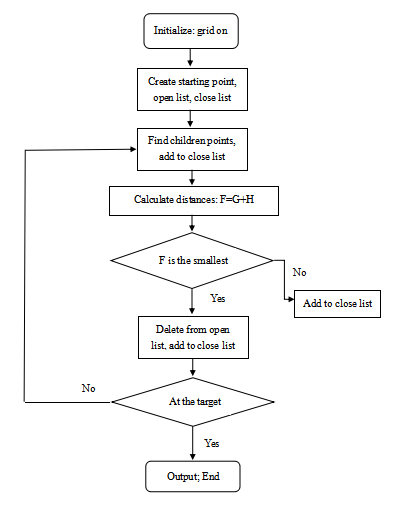
\includegraphics[width=3.5in]{figure2}
\label:{figure 2}
\end{figure}

\item{ High Level Pseudo Code System Description. }

\begin{lstlisting}[language={[ANSI]C}, title=pseudo code of A* algorithm, keywordstyle=\color{blue!70},
commentstyle=\color{red!50!green!50!blue!50},frame=shadowbox,rulesepcolor=\color{red!20!green!20!blue!20},
numbers=left,numberstyle=\tiny]
Astar(){
    Table open,close;
    inject(s,open);//s is the starting point
    while(open!=NULL){
        node n=ExtractMin(open);
        if(n==target){
            break;
        }
        for each x as child of n{
            if(x in open){
                if(cost(x)<cost(open)){
                    x.parent=n;
                    update(open);
                }
            }
            if(x in close){
                if(cost(x)<cost(close)){
                    x.parent=n;
                    update(close);
                    inject(x,open)
                }
            }
            else{
                x.parent=n;
                calculate cost(x);
                inject(x,open)
            }
        }
        inject(n,close);
        sort(open);
    }
    path p;
    for node x=target to s{
        p.generate(x)//starting from the target point and follows its parent node until the starting point
    }
    return p;
 }
\end{lstlisting}

\item{Algorithms and  Data Structures. }
The major algorithm is A* algorithm, which is a heuristic algorithm widely used in path finding and graph traversal. This project will use this algorithm to visualize the process of solving a "eight-figure puzzle" game.
The main data structures include array, hash table, priority queue, and probably object-oriented programming.
\end{itemize}

\begin{itemize}
\item{  Flow Diagram Major Constraints.}
Please insert here the integrity constraints:
\begin{itemize}
\item{ Integrity Constraint 1 }

Username, password: varchar(20), not replicable, not null

User type: one of "original", "advanced" and "administrator"
\end{itemize}
\begin{itemize}
\item{ Integrity Constraint 2 }

step speed: float number
\end{itemize}
\end{itemize}



%\subsection{Stage3 - The Implementation Stage. }\label{sec: 3 The Implementation Stage.}
%%%%%%%%%%%%%%%%%%%%%%%%%%%%%%%%%%%%%%%%%%%%%%%%%%%%%%%%%%%%%%%%%%%%%%%%%%%%%%%%%%%%%%%%%
%\input{Stage3.tex}

%\subsection{Stage4 -	User Interface. }\label{sec: 4. User Interface.}
%%%%%%%%%%%%%%%%%%%%%%%%%%%%%%%%%%%%%%%%%%%%%%%%%%%%%%%%%%%%%%%%%%%%%%%%%%%%%%%%%%%%%%%%%%%%%%%%%%%%%%%%%%
%\input{Stage4.tex}

%\section{Project Highlights.}\label{sec:7. Project Highlights.}
%%%%%%%%%%%%%%%%%%%%%%%%%%%%%%%%%%%%%%%%%%%%%%%%%%%%%%%%%%%%%%%%%%%%%%%%%%%%%%%%%%%%%%%%%%%%%%%%%%%%%%%%%%
%\input{Highlights.tex}


\bibliographystyle{IEEEtran}
%\bibliography{IEEEabrv,bib_queyroi_abello2013}
%\bibliography{bib_queyroi_abello2013}

\end{document}


